\begin{figure}[h]
\centering
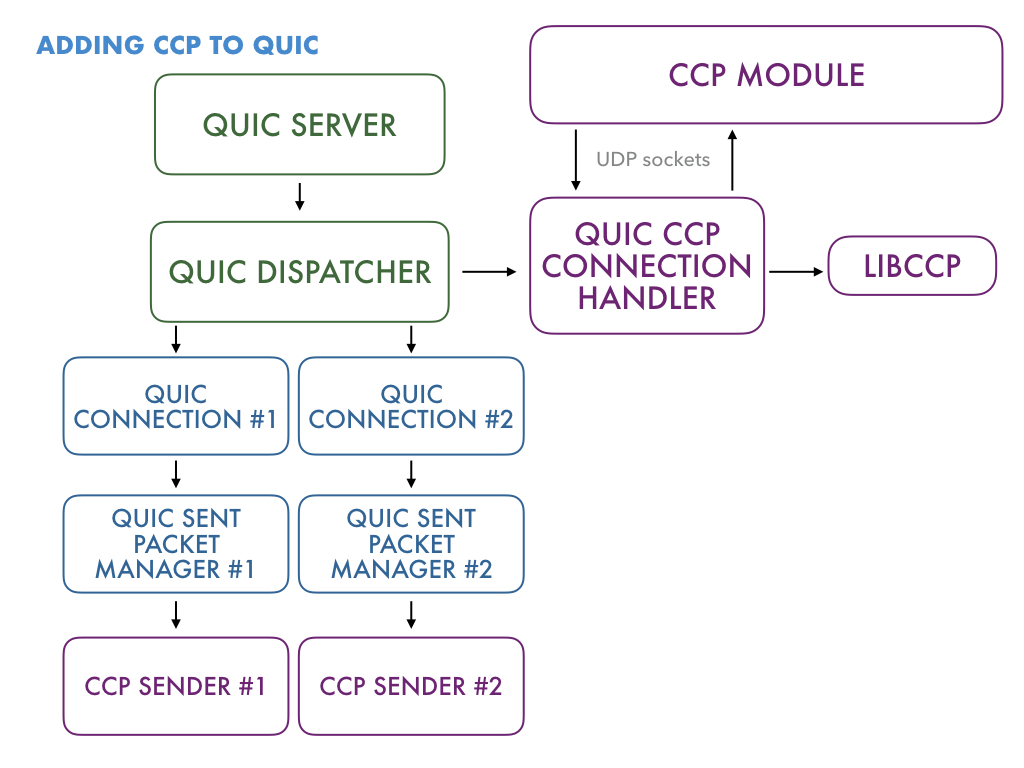
\includegraphics[scale=.45]{implementation/ccpquic_diagram}
\caption{The \ct{QuicCCPConnectionHandler} class implements the \libccp API. It provides the time related functions through the C++ standard library's wall clock time. By passing in the pointer to the specific \ct{QuicConnection} object to a call to \ct{Set\_Congestion\_Window}, the CCP connection handler propagates the instruction down to the specific CCP sender object.}
\label{fig:ccpquic_diagram}
\end{figure}

